\chapter{相关技术和方法}
\markboth{正文}{正文}

随着深度学习和神经网络技术的发展,计算机视觉相关任务的性能获得了显著提升。这些任务的发展不仅得益于主干网络(Backbone)令人瞩目的特征提取能力,也受益于多个领域的技术和方法。图像超分辨率重建任务作为计算机视觉领域的一个重要分支,随着相关理论和技术的不断丰富和发展,研究者已逐步认知到与该任务相关的关键问题和难点问题,并借鉴和采用了相应的技术和方法以提升图像超分辨率重建任务的性能。在本章中,将主要介绍计算机视觉任务的通用方法和与图像超分辨率重建任务密切相关的方法,包括:卷积神经网络 \cite{qiu2020nndl}、编码器-解码器架构 \cite{DBLP:conf/eccv/NewellYD16}、注意力机制 \cite{DBLP:conf/eccv/WooPLK18}、多尺度理论 \cite{DBLP:journals/tip/YeSWYXLL20} 和像素重组 \cite{DBLP:conf/cvpr/ShiCHTABRW16}。

\section{卷积神经网络}
卷积神经网络(Convolutional Neural Network, CNN)是一种具有稀疏连接,权重共享等特点的深层神经网络,一般由若干卷积层(Convolutional Layer)、池化层(Pooling Layer)、激活函数(Activation Function)、批正则化层(Batch Normalization Layer)和全连接层(Full Connected Layer)交叉堆叠而成。网络通过对损失函数(Loss Function)的优化(Optimizer)实现参数的更新,从而获得最优的参数。

\subsection{卷积}

顾名思义,卷积神经网络的核心是卷积操作。卷积,可以看作是特征提取器,图像经过卷积运算后可以得到图像的特征映射,如图 \ref{fig:fig2-1} 所示。给定一个图像(或特征图) $X\in R^{W\times H}$ 和一个卷积核 $\omega\in R^{w\times h}$ ,其中 $W\times H$ 分别为图像的宽度和高度和,$w\times h$ 分别为卷积核的宽度和高度,且一般有 $w\ll W$,$h\ll H$。则卷积操作可定义为式 \ref{equ:equ2-1}。

\begin{equation}
	y_{ij}=\sum_{u=1}^{w}\sum_{v=1}^{H}\omega_{uv}x_{i-u+1,j-v+1}
	\label{equ:equ2-1}
\end{equation}

\noindent 式中,$y_{ij}$ —— 卷积的输出;\newline
\indent\quad $\omega_{uv}$ —— 卷积核的一个位置;\newline
\indent\quad $x_{i+u-1,j+v-1}$ —— 图像中与卷积核位置相对应的像素。

\newpage

\begin{figure}[!htbp]
	\centering
	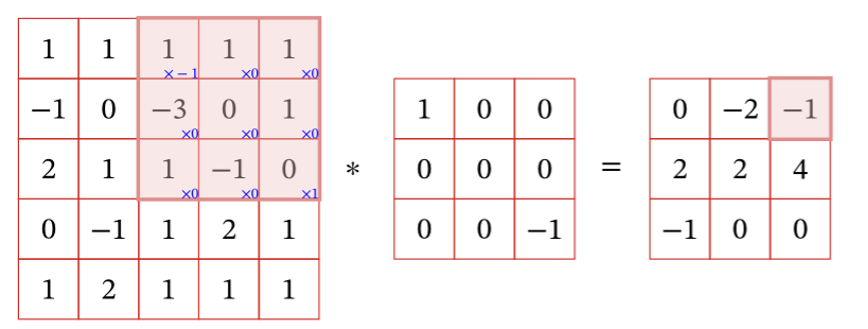
\includegraphics{figures/2.png}
	\caption{卷积示例图}
	\label{fig:fig2-1}
\end{figure}

如图所示,第一个矩阵为参与卷积操作的图像(或特征图),第二个矩阵为大小为 $3\ \times3$ 的卷积核,第三个矩阵则为将卷积核作用于图像(或特征图)的输出。在卷积操作时,卷积核被用于在图像(或特征图)上滑动以计算得到新的特征。可以看到,当卷积核滑动到图像(或特征图)的右上角时,输出特征对应位置(即第三个矩阵右上角位置)的像素值为卷积核窗口中所有像素的平均值。在实际计算卷积时,会对卷积核进行翻转。

为了更加灵活地提取特征,通常会引入卷积核的滑动步长(Stride)和填充(Padding)。卷积核在图像或特征图上的滑动是从左上方开始,按照从左至右、自上而下的准则进行,每次滑动的行数(或列数)称为滑动步长。填充则是指在图像或特征图的四周填充元素(通常是0)。

如图 \ref{fig:fig2-1} 所示,下方的蓝色矩阵为输入的图像(或特征图),上方的绿色矩阵为卷积操作提取的特征。第一行为步长为1且不进行填充的卷积操作;第二行为步长为2且不进行填充的卷积操作,此时卷积核在图像(或特征图)上滑动时每次移动两个像素;第三行为步长为1而填充为2卷积操作,蓝色图像(或特征图)周围的虚线矩形即为填充的元素。

从图中也可以看到,卷积提取的特征图大小不仅与输入图像(或特征图)和卷积核的大小有关,而且与卷积核的滑动步长核填充元素的数量也有关系。这一关系即为式 \ref{equ:equ2-2} 和式 \ref{equ:equ2-3}。

\begin{equation}
	W_{out}=\left\lceil\frac{W_{in}+2\times p-w}{s}\right\rceil+1
	\label{equ:equ2-2}
\end{equation}
\vspace{0.7cm}
\begin{equation}
	H_{out}=\left\lceil\frac{H_{in}+2\times p-h}{s}\right\rceil+1
	\label{equ:equ2-3}
	\vspace{0.3cm}
\end{equation}

\noindent 式中,$W_{out}$,$H_{out}$ —— 输出特征图的宽度和高度;\newline
\indent\quad $W_{in}$,$H_{in}$ —— 输入图像(或特征图)的宽度和高度;\newline
\indent\quad $w$,$h$ —— 卷积核的宽度和高度;\newline
\indent\quad $p$,$s$ —— 填充大小和步长。

\begin{figure}[!htbp]
	\centering
	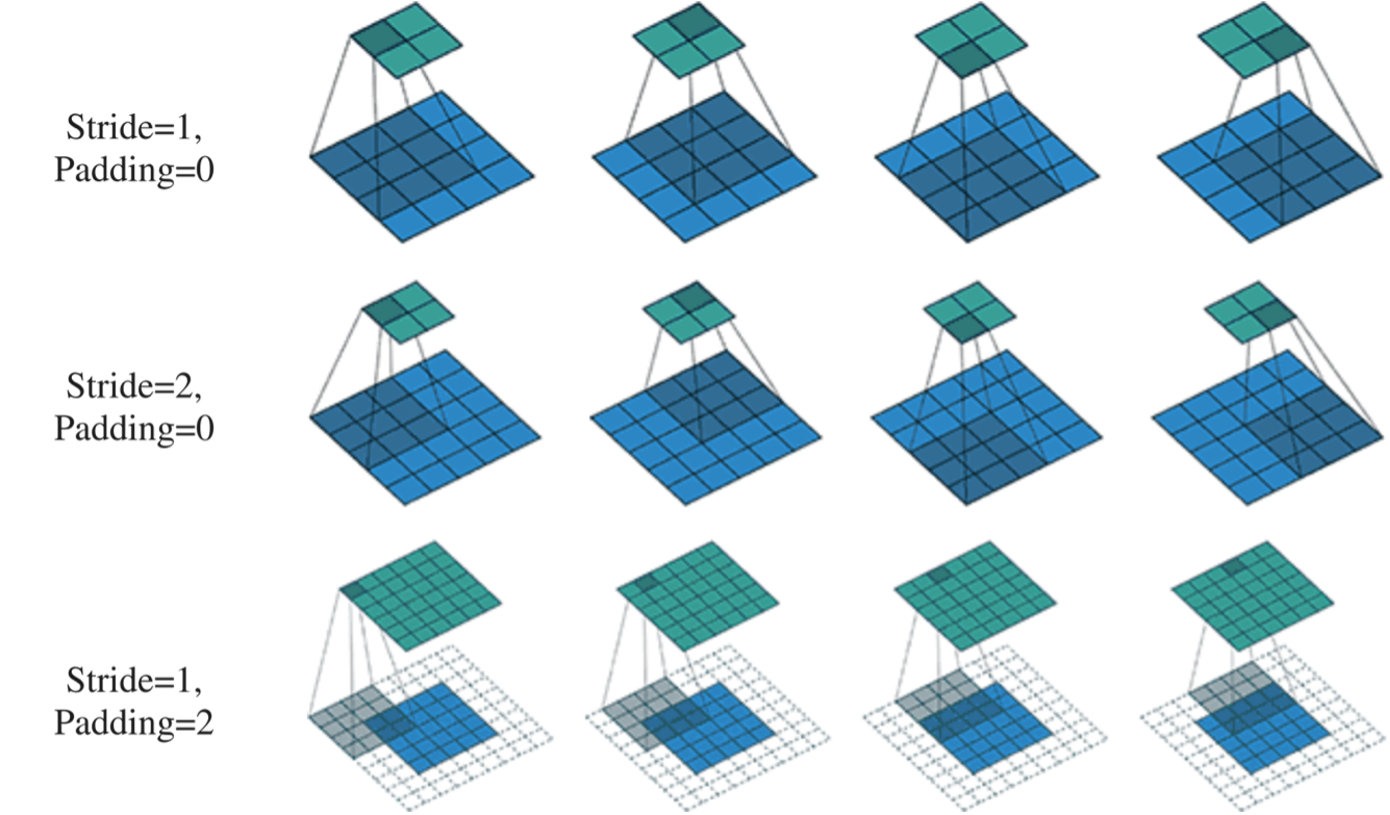
\includegraphics{figures/3.png}
	\caption{不同滑动步长和填充的卷积示例图}
	\label{fig:fig2-2}
\end{figure}

对于一幅图像来讲,除了目前已经提到的宽度和高度两个维度而言,还有颜色通道(例如,彩色图像有三个通道,深度图像只有深度一个通道),即给定一个图像(或特征图) $X\in R^{W\times H\times C}$ 和一个卷积核 $w\in R^{w\times h\times c}$,其中 $C$ 和 $c$ 分别为图像和卷积核的通道数,一般有 $C=c$。则卷积可以定义为对应通道的图像(或特征图)与卷积核进行卷积操作后相加,如图 \ref{fig:fig2-3} 所示。

\begin{figure}[!htbp]
	\centering
	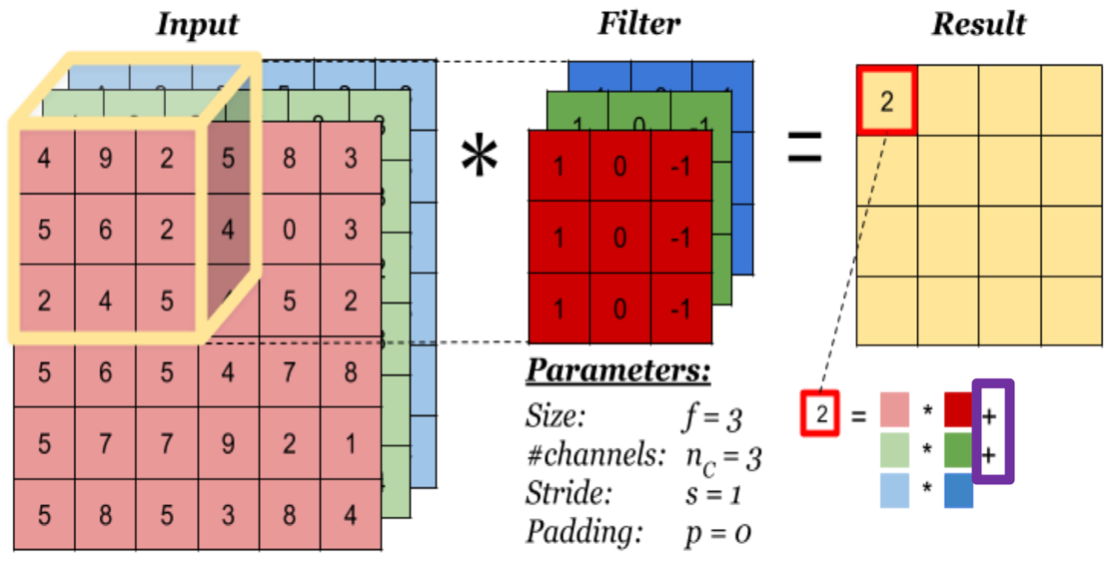
\includegraphics{figures/4.png}
	\caption{三通道彩色图像卷积示例图}
	\label{fig:fig2-3}
\end{figure}

图 \ref{fig:fig2-3} 中,左侧为输入的RGB三通道图像,中间为与图像通道数相同的卷积核,在对应颜色通道进行卷积操作后,将三个通道的结果相加(如图中右下角所示),即为输出特征对应位置的值。

\subsection{激活函数}

卷积操作在提取特征的过程中,能有效去除图像(或特征图)中的噪声。通过卷积层的堆叠,特征图的大小逐渐下降,感受野逐渐增大,特征包含的信息逐渐从低级的结构信息转变为高级的语义信息。但由于卷积操作的线性特征,即使是堆叠的卷积操作仍然面临着表示能力不足的问题。因而引入了激活函数这一非线性操作以增强模型的特征表示能力。此外,由于反向梯度传播在神经网络训练中取得的成功,决定了激活函数必须具备可导的特质。常用的激活函数有 Sigmoid, Tanh, ReLU, Leaky ReLU,其函数图像如图 \ref{fig:fig2-4} 所示。

\begin{figure}[!htbp]
	\centering
	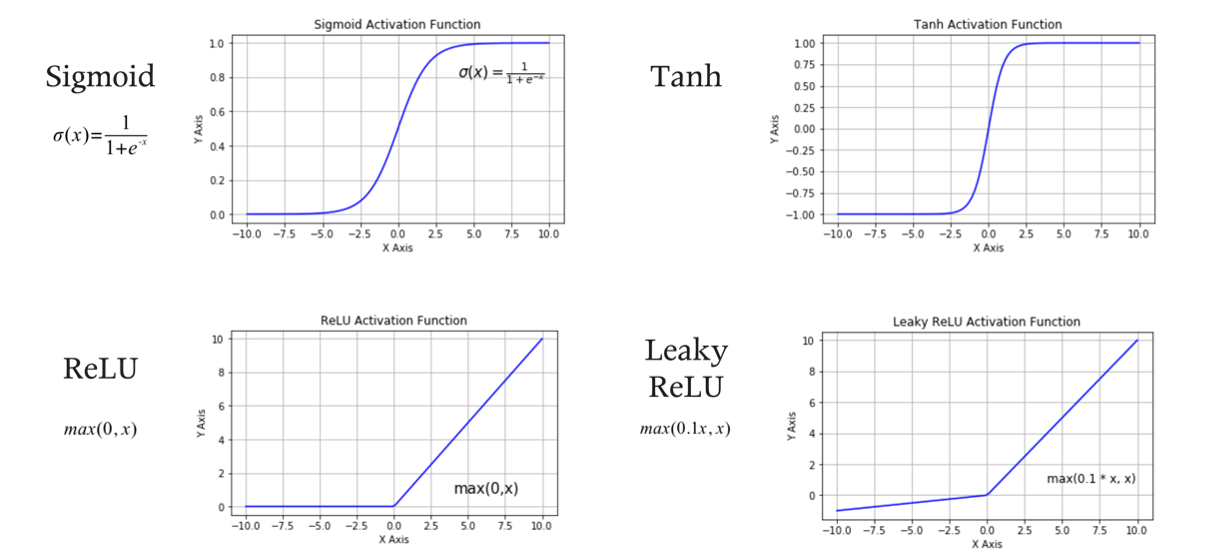
\includegraphics{figures/5.png}
	\caption{常用激活函数及其函数图像}
	\label{fig:fig2-4}
\end{figure}

\subsection{池化}

卷积层由于其稀疏连接的特性可以显著减少网络中连接的数量,但神经元的数量却并没有发生变化。可以预见的是,仅包含卷积层和激活函数的神经网络会导致分类器的输入维度很高。池化层(一种降采样)正是为解决这样的问题而被引入了卷积神经网络,以实现降低特征数量和减少参数量的效果。此外,卷积操作可以精确地找到像素变化的位置,但在实际的图像数据中,研究对象并不总是出现在固定位置,可能会导致相同的特征经过卷积后的输出不同,给下游任务带来不便。以人的视觉为例,我们可以从一张包含狗的降采样图像中识别出图像内容,这说明压缩后的图像仍保留了狗最关键的特征,而图像降质时丢掉的是一些无伤大雅的信息,最能描述狗的尺度不变特征则仍然保留在图像中。因此,池化层还有一个作用是特征选择,减少由于像素位置变化造成的特征变化。一般所使用的池化层为最大池化(Max-pooling)和平均池化(Average-pooling)两类。最大池化如图 \ref{fig:fig2-5} 所示。

\begin{figure}[!htbp]
	\centering
	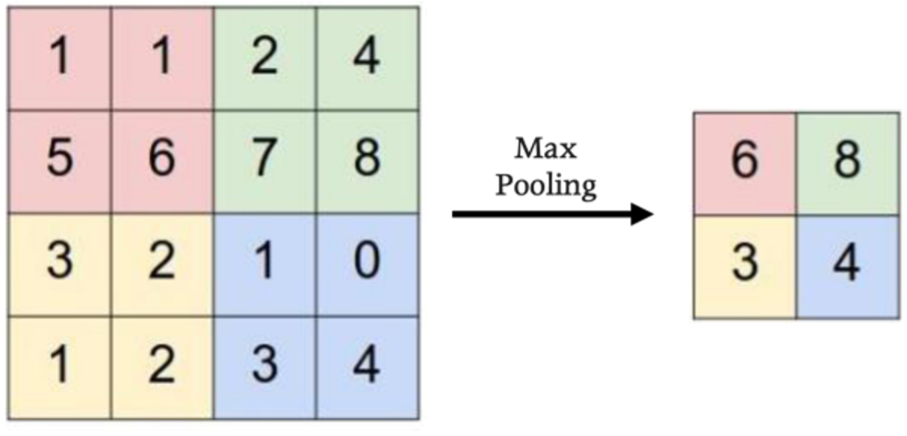
\includegraphics{figures/6.png}
	\caption{最大池化示例图}
	\label{fig:fig2-5}
\end{figure}

\newpage
可以看到,最大池化是将输入的图像划分为若干个(图中为4个)矩形区域,然后分别取各个区域的最大值得到的。而平均池化则是取各个区域的平均值。

\subsection{正则化}

卷积神经网络在训练时通过误差的反向传播和梯度下降来不断更新网络的参数。而随着前面层在训练过程中对参数的更新,导致了传输到后面层作为输入数据的分布发生了变化。也就是说,在训练过程中,除了输入层之外,网络每一层输入数据的分布一直在发生变化,这一问题被称为内部协变量位移(Internal Covariate Shift)。而批正则化(或批量归一化)可以用于解决这一问题。批正则化可以对网络中任意一层进行归一化处理,保证每一层的数据都处于同一分布。这一算法可以定义为式 \ref{equ:equ2-4}。

\vspace{0.5cm}
\begin{equation}
	{\hat{x}}^{\left(k\right)}=\frac{x^{\left(k\right)}-E\left[x^{\left(k\right)}\right]}{\sqrt{Var\left[x^{\left(k\right)}\right]}}
	\label{equ:equ2-4}
	\vspace{0.3cm}
\end{equation}

\noindent 式中,$x^{\left(k\right)}$ —— 输入数据第 $k$ 个维度的值;\newline
\indent\quad      $E\left[x^{\left(k\right)}\right]$ —— 第 $k$ 个维度的期望;\newline
\indent\quad       $\sqrt{Var\left[x^{\left(k\right)}\right]}$ —— 第 $k$ 个维度的方差。

\subsection{全连接}

综上,一般卷积神经网络的结构如图 \ref{fig:fig2-6} 所示。卷积神经网络中一般由 $N$ 个连续的卷积块堆叠而成,最后有 $F$ 个连续的全连接层($N$ 的取值可以很大,而 $F$ 一般为0 $\sim$ 2)。其中,每个卷积块由 $C$ 个卷积层(包括激活函数)和 $P$ 个池化层($M$ 的取值通常为2 $\sim$ 5,而 $b$ 为0或1)串联组成。

\begin{figure}[!htbp]
	\centering
	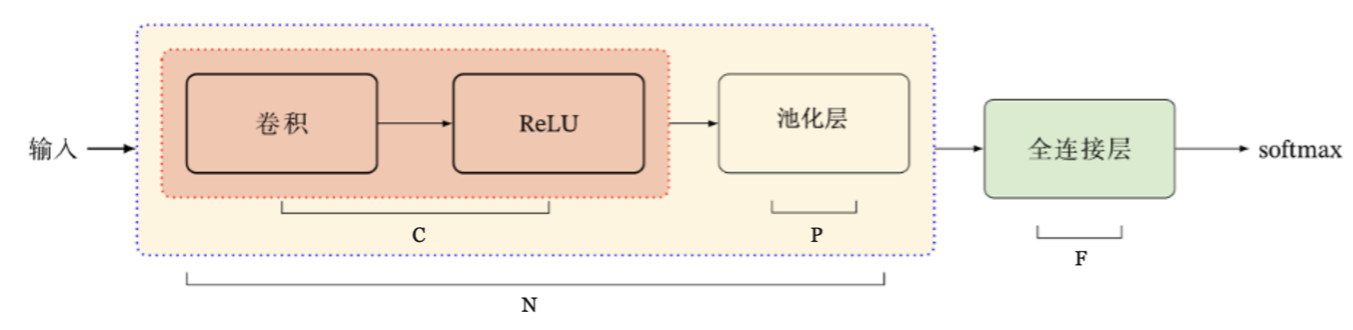
\includegraphics{figures/7.png}
	\caption{典型的卷积神经网络结构图}
	\label{fig:fig2-6}
\end{figure}

\newpage
全连接层在卷积神经网络中一般用于分类。在通过连续的卷积层和激活函数捕捉到了原始图像的特征表示后,全连接层将提取的特征聚合并转换到最终的样本空间,如图 \ref{fig:fig2-7} 所示。

\begin{figure}[!htbp]
	\centering
	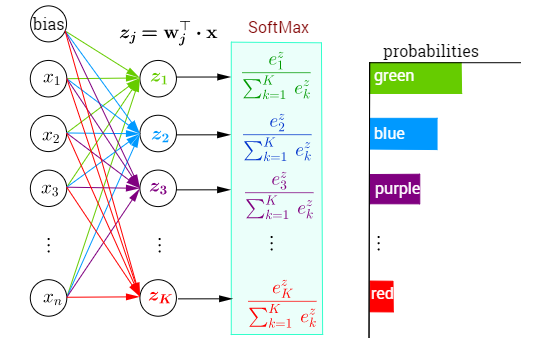
\includegraphics[scale=0.55]{figures/8.png}
	\caption{全连接层示例图}
	\label{fig:fig2-7}
\end{figure}

顾名思义,与卷积的稀疏连接不通,从图 \ref{fig:fig2-7} 可以看到,全连接层中的每一个“神经元”都与上一层中的所有“神经元”相连。全连接层将网络提取的二维图像特征映射为样本标记类别得分(取值范围为 $\left[-\infty,+\infty\right]$) 的一维向量,而通常网络的全连接层后会紧跟一个 Softmax 操作,将类别得分转换为概率以便于后续操作。 Softmax 操作的定义为式 \ref{equ:equ2-5}。

\begin{equation}
	{\hat{y}}_i=softmax(z_i)=\frac{e^{z_i}}{\sum_{K} e^{z_i}}
	\label{equ:equ2-5}
	\vspace{0.3cm}
\end{equation}

\noindent 式中,$z_i$, ${\hat{y}}_i$ —— 第 $i$ 个类别的得分和对应的概率;\newline
\indent\quad $K$ —— 分类的类别数或全连接层的输出维度。

\subsection{其他卷积}

前文介绍的卷积实现了低层特征到高层特征的转换,同样,也可以实现特征维度间的转换。例如,通过三个卷积核可以实现将通道数为5的特征转变为通道数为3的特征。而在一些明确的任务(如图像的超分辨率重建)中,存在着将特征从低层到高层进行转换的需要,也就是对特征图或图像进行“上采样”。转置卷积(Transposed Convolution)也被称为反卷积(Deconvolution),通过填充扩大特征,实现了由低分辨率特征图到高分辨率特征图的操作。如图 \ref{fig:fig2-8}(右)所示。

\begin{figure}[!htbp]
	\vspace{-0.5cm}  %调整图片与上文的垂直距离
	\centering
	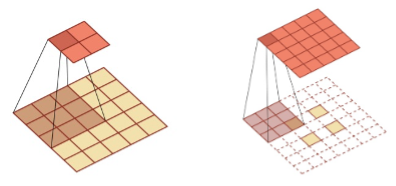
\includegraphics{figures/9.png}
	\caption{转置卷积(反卷积)示例图}
	\label{fig:fig2-8}
\end{figure}

图中下方的黄色矩阵为输入图像(或特征图),上方的橙红色矩阵为“卷积”操作的输出。可以看到与左侧卷积操作不同的是,反卷积的输出比输入图像(或特征)在空间维度上大,从而可以承担图像超分辨率重建任务中上采样的工作。

\section{编码器-解码器框架}

编码器-解码器(Encoder-Decoder)框架最先被应用于自然语言处理领域的有关任务,如机器翻译等。编码器是以训练数据作为输入,特征张量作为输出的网络。这些特征张量就是输入的信息和特征嵌入到其他表示空间的内容。解码器通常是一个与编码器结构相似(或与特定任务有关的结构)但方向相反的网络结构,它从编码器获取特征张量,然后输出与实际输入或预期输出同一表示空间的结果。近年来,编码器-解码器架构作为一类深度学习框架,也被广泛应用于计算机视觉领域,并在图像分割、光流估计、深度估计等任务取得了成功。也就是说,编码器的输入可以是文字,图像或视频数据,而具体的模型可以采用卷积神经网络,循环神经网络等。以卷积神经网络作为编码器和解码器的模型通常如图 \ref{fig:fig2-9} 所示,左侧为网络的编码器,以彩色图像作为输入并生成图像的特征,右侧为网络的解码器,以编码器提取的特征作为输入,然后将特征映射到预期输出的表示空间,这里为图像的语义标签。

\begin{figure}[!htbp]
	\centering
	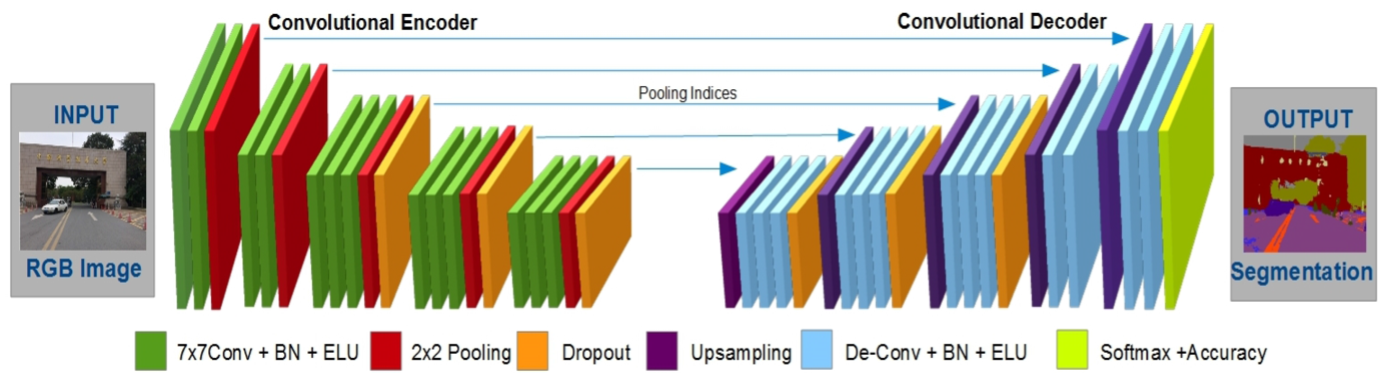
\includegraphics[scale=0.98]{figures/10.png}
	\caption{编码器-解码器框架示例图}
	\label{fig:fig2-9}
\end{figure}

\section{注意力机制}

在观看一张图片时,人们并不能立即接收图片的全部内容,而是往往将注意力集中在了一些显著位置。图 \ref{fig:fig2-10} 所示的是对人浏览报纸时注意力的模拟,可以看到注意力集中在图像中的显眼目标(如标题)或直观且包含大量信息(如图片)的位置。

\begin{figure}[!htbp]
	\centering
	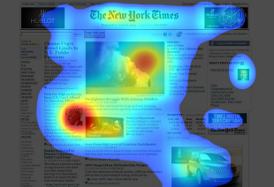
\includegraphics{figures/11.png}
	\caption{注意力示例图}
	\label{fig:fig2-10}
\end{figure}

同理,注意力机制的作用便是帮助模型对输入数据赋予不同的权重,使得模型关注输入数据中更加重要和关键的信息。此外,注意力机制还可以使得模型在做出准确判断的同时而不带来巨大的计算和存储开销。

基于项的注意力和基于位置的注意力根据其不同的输入形式而有所不同。基于项的注意力用于在输入中已经给出或可以提取得到项(如向量,矩阵等)的任务。而基于位置的注意力则用于从输入难以获取项的任务,因而一般以特征图作为输入,或在输入前对该特征图进行一定的变换使得网络在后续阶段可以更好地利用它。

根据学习机制的不同,注意力可以分为软注意力和强注意力。软注意力通常关注区域或通道,且会对所有输入进行线性组合。因此,软注意力一般由端到端的结构(或网络)生成,即可以通过梯度下降的方法学习得到。而硬注意力则是根据输入数据的分布随机进行选择,也就是说,强注意力是不可微的。强注意力的训练过程一般是通过强化学习(Reinforcement Learning) 的收益函数(Reward)来进行激励,从而让模型更加关注数据的局部细节。

而按照注意力域的不同,注意力又可以分为通道注意力(Channel Attention),空间注意力(Spatial Attention)和混合注意力(Mixed Attention)。下面将分别对使用通道注意力和空间注意力思想的经典网络结构进行介绍。

\newpage

\subsection{通道注意力}

卷积神经网络通过卷积等操作提取包含空间和通道信息的特征,现有很多针对网络的研究是从增强特征的空间表示能力的角度来提升网络的性能。而通道注意力则是对特征通道间的关系进行建模,让网络可以自动地学习不同通道的重要性。压缩-激励网络(Squeeze-and-Excitation Network, SENet) \cite{DBLP:conf/cvpr/HuSS18} 是一个利用通道注意力思想的经典网络。如图 \ref{fig:fig2-11} 所示,其操作是对特征图进行空间维度的压缩,从而将具有通道级特征响应的全局分布嵌入一个一维向量中,并通过激励操作获得每个通道权重的集合,然后分别与对应通道相乘,从而得到施加注意力的结果。

\begin{figure}[!htbp]
	\centering
	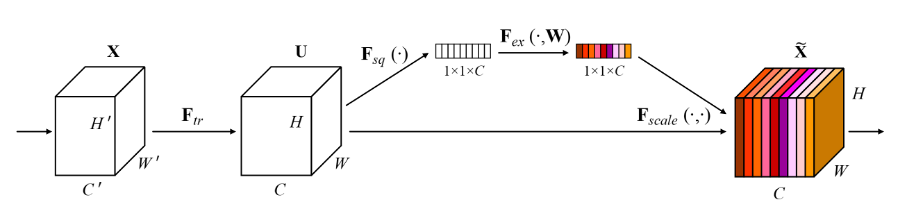
\includegraphics[scale=0.98]{figures/12.png}
	\caption{压缩-激励模块结构图}
	\label{fig:fig2-11}
\end{figure}

\subsection{空间注意力}

对于卷积神经网络所提取的特征图 $F\in R^{W\times H\times C}$,$W$,$H$,$C$ 分别代表特征图的宽度、高度和通道数量。$W\times H$ 可以看作一个平面,其中的每个值代表的当前位置的信息。尽管经过卷积等操作,这个位置已经不再是原始图像像素的位置,但是依然是一种位置信息。与通道注意力类似,如果可以学习到一个 $W\times H$ 的权重矩阵,将矩阵的每一个元素与特征图所有通道对应位置的元素相乘,就相当于对空间位置进行了加权,即对特征图施加了空间注意力。换言之,空间注意力是对特征图的每个位置进行加权调整,促使模型关注到更加值得关注的区域。

\begin{figure}[!htbp]
	\centering
	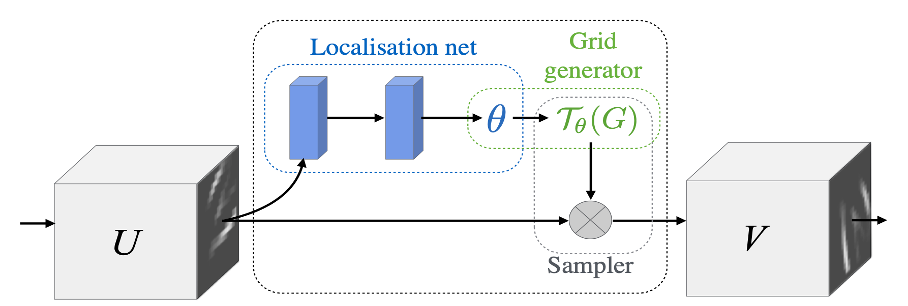
\includegraphics[scale=0.95]{figures/13.png}
	\caption{空间转换模块结构图}
	\label{fig:fig2-12}
\end{figure}

空间转换网络(Spatial Transformer Networks, STN)\cite{DBLP:conf/nips/JaderbergSZK15} 是一个利用空间注意力思想的经典网络,其动机是通过设计的模块让网络学习一种变换,这种变换可以将进行了仿射变换的目标进行矫正。通俗而言,就是将图像或特征的空间信息做对应的变换,从而将关键信息提取出来,即找出图片信息中需要被关注的区域。如图 \ref{fig:fig2-12},这种变换的学习主要是通过局部网络(Localisation Network)、参数化网格采样(Parameterised Sampling Grid)和差分图像采样(Differentiable Image Sampling)实现的,分别用于变换参数的预测、变换前后图片坐标的映射和像素的采集。

\section{多尺度机制}

在计算机视觉任务中,尺度微小的物体与超大的物体对模型的性能有着很大的影响。目标特征在图像逐层经过卷积神经网络的过程中被提取出来,卷积层的感受野也随着网络的深入不断变大。但感受野过大,提取的特征会包含冗余的无效信息,而感受野太小,就只能捕获到图像的局部特征。为了实现精确的目标检测、识别或是像素级回归,就需要多尺度技术来增强网络的特征表示能力。多尺度机制就是对图像进行不同粒度的采样,模型在不同的尺度下可以捕捉到不同的特征。根据网络设计的不同可以分为多尺度输入、多尺度特征融合和多尺度预测融合。

多尺度输入就是将不同尺度的图像作为输入,也就是图像金字塔。多尺度特征融合通常有两种结构,一种是多分支并行的结构(如 Inception 模块),通过多分支在同一层提取不同粒度大小的特征,融合后传递到网络的下一层。并行的结构可以更加灵活地平衡计算量,并提高模型的特征表示能力。另一种是跨层连接的串行结构(如全卷积神经网络),这种结构的实现方式是通过跳连接将不同层的特征进行融合。串行的结构可以帮助边界敏感任务(如语义分割)更好地捕捉边界细节。图 \ref{fig:fig2-13} (左)为并行分支的多尺度特征融合结构,图 \ref{fig:fig2-13} (右)为串行跳层连接的多尺度特征融合结构。

\begin{figure}[!htbp]
	\centering
	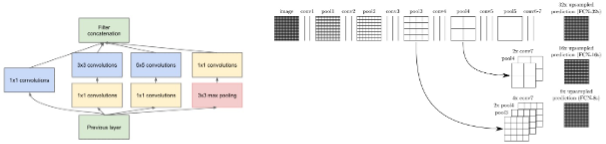
\includegraphics{figures/14.png}
	\caption{多尺度特征融合结构示例图}
	\label{fig:fig2-13}
\end{figure}

多尺度预测融合是根据不同尺度的特征进行预测,然后将不同尺度的结果融合。但多尺度输入结构独立地在不同尺度的图片上进行计算,造成了巨大的计算开销,而多尺度特征融合与多尺度预测融合结构由于缺乏对特征金字塔的充分利用,其准确度仍有待提升。特征金字塔网络则是结合了多尺度特征融合与多尺度预测融合的特点,在每个分辨率的特征图与前一层上采样后的特征图逐像素相加,从而使得每一层用于预测的特征图融合了不同分辨率和不同语义信息的特征。与其他的多尺度方法相比,特征金字塔的每一层的特征都具有合适的分辨率以及丰富的语义。特征金字塔网络的结构如图 \ref{fig:fig2-14} 所示。

\begin{figure}[!htbp]
	\centering
	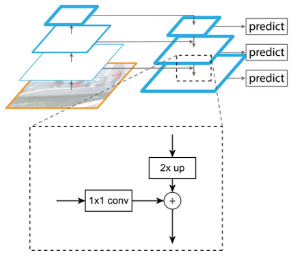
\includegraphics{figures/15.png}
	\caption{特征金字塔网络结构图}
	\label{fig:fig2-14}
\end{figure}

\section{像素重组}

像素重组(PixelShuffle)以低分辨的特征图左为输入,通过卷积和特征通道间的重组得到高分辨率的特征图,从而可以有效地解决图像的超分辨率重建问题。如图 \ref{fig:fig2-15} 所示,在隐藏层中进行的是对图像的特征提取,紧随其后的一层生成 $w\times h\times r^2$ 的特征图,其中,$w$ 、$h$、$r^2$ 分别为特征图的宽度、高度和通道数量,$r$ 为图像超分辨率重建中的上采样因子。像素重组作用于这一特征图并重新组合为宽度和高度分别为 $w\times r$,$r\times h$ 的上采样特征图。具体而言,像素重组就是把低分辨特征图的一个像素划分为 $r$ 个“亚像素”,然后将特征图 $r$ 个通道对应位置的值按照预先制定的规则来填充划分出的“亚像素”。在每个低分辨特征图像素划分出的“亚像素”被填满后,就完成了像素重组。在填充过程中,像素重组层可以更新 $r^2$ 个通道的权重以优化生成的高分辨率特征图。

\begin{figure}[!htbp]
	\centering
	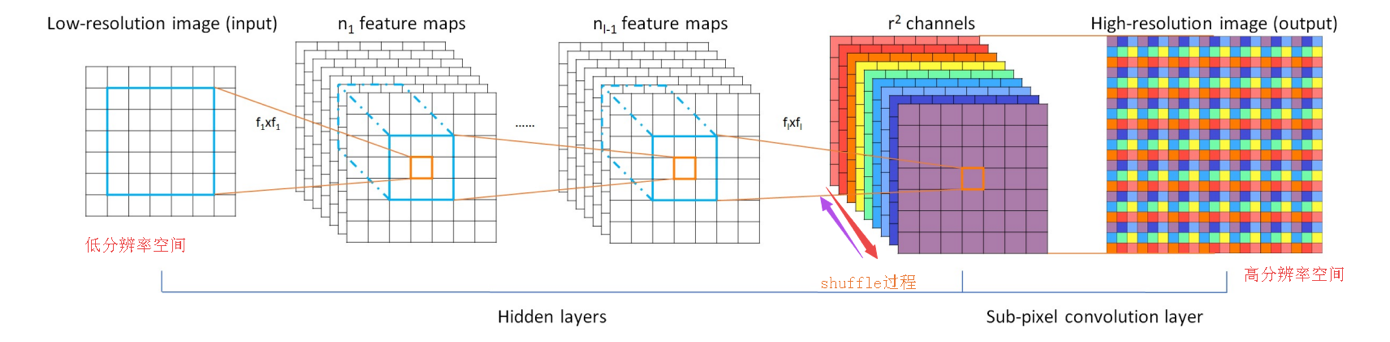
\includegraphics{figures/16.png}
	\caption{像素重组结构图}
	\label{fig:fig2-15}
\end{figure}


\section{本章小结}
本章介绍了本文所提出的单目深度估计和深度图像超分辨率重建联合学习网络所使用的技术和方法。本章所介绍的内容主要分为计算机视觉任务的通用方法和与图像超分辨率重建任务密切相关的方法,其中计算机视觉任务通用方法即为卷积神经网络。而在后续介绍与图像超分辨率重建任务相关的技术时,如多尺度机制,像素重组等,则是围绕着这些技术与卷积神经网络的相关性来引入和展开的。也就是说,卷积神经网络是计算机视觉任务的技术基石,而其他相关理论和方法则是推动细分任务发展的重要工具。综上,本文提出的单目深度估计和深度图像超分辨率重建联合学习网络整体上采用编码器-解码器框架,以卷积神经网络作为网络设计的原型,辅助以注意力机制、多尺度机制和像素重组等方法,从而构成了完整的网络设计。 

